\documentclass{beamer}
\usepackage[utf8]{inputenc}
\usepackage[T1]{fontenc}
\usepackage{setspace}
\usepackage{gensymb}
\usepackage{amsmath}
\usepackage{amssymb}
\usepackage{bm}
\usepackage{graphicx}
\usepackage{hyperref}
\usepackage{listings}
\usepackage{xcolor}
\usepackage{array}
\usepackage{calc}
\usepackage{hhline}
\usepackage{ifthen}
\usepackage{textcomp}

\singlespacing
\usetheme{CambridgeUS}

% Robust listings configuration
\lstset{
    basicstyle=\ttfamily\footnotesize,
    breaklines=true,
    postbreak={\mbox{\textcolor{red}{\tiny$\hookrightarrow$}\space}},
    columns=fullflexible,
    keepspaces=true,
    showstringspaces=false,
    upquote=true,
    literate={~}{{\textasciitilde}}1
}

\title[Digital Clock Implementation]{Digital Clock Implementation using Arduino with Multiplexing and Editing Features}
\author{Dhawal}
\institute[IITH]{Department of Electrical Engineering\\Indian Institute of Technology Hyderabad\\Email: ee24btech11015@iith.ac.in}
\date{}

\begin{document}

\begin{frame}
    \titlepage
\centering
Electrical Engineering Department\\
Indian Institute of Technology, Hyderabad
\end{frame}

\begin{frame}{Outline}
    \tableofcontents
\end{frame}

\section{Introduction}
\begin{frame}{Introduction}
\begin{itemize}
    \item Digital clock system with editing features using Arduino
    \item Multiplexing six 7-segment displays using minimal I/O pins
    \item Pause/play functionality and digit-by-digit editing
    \item Boolean logic for increment/decrement and constraints for each digit
\end{itemize}
\end{frame}

\section{Components}
\begin{frame}{Components List}
\centering
\begin{tabular}{|l|c|c|}
\hline
Component & Value & Quantity\\
\hline
Arduino Uno & & 1\\
USB Cable & Type B & 1\\
Seven Segment Display & Common Cathode & 6\\
Push Buttons & & 4\\
IC 7447 & & 1\\
Jumper Wires & M-M & 16\\
Breadboard & & 1\\
Resistors & 220$\Omega$ & 7\\
Resistors & 10$k\Omega$ & 4\\
\hline
\end{tabular}
\end{frame}

\section{Circuit Connections}
\begin{frame}{Arduino Pin Connections}
\centering
\begin{tabular}{|c|c|c|}
\hline
Item & Arduino Pin & Function\\
\hline
Button 1 & D10 & Edit Mode Toggle\\
Button 2 & D11 & Next Digit Selection\\
Button 3 & D12 & Increment Digit\\
Button 4 & D13 & Decrement Digit\\
IC 7447 Pin 7 & D0 & BCD Bit 0 (A)\\
IC 7447 Pin 1 & D1 & BCD Bit 1 (B)\\
IC 7447 Pin 2 & D2 & BCD Bit 2 (C)\\
IC 7447 Pin 6 & D3 & BCD Bit 3 (D)\\
Display 1 & D4 & Hours Tens Digit\\
Display 2 & D5 & Hours Units Digit\\
Display 3 & D6 & Minutes Tens Digit\\
Display 4 & D7 & Minutes Units Digit\\
Display 5 & D8 & Seconds Tens Digit\\
Display 6 & D9 & Seconds Units Digit\\
\hline
\end{tabular}
\end{frame}

\section{Multiplexing Technique}
\begin{frame}{Multiplexing}
\begin{itemize}
    \item All BCD inputs shared among six 7-segment displays
    \item Arduino controls enable pins D4-D9
    \item Each digit displayed for 1ms → appears continuous
    \item Saves I/O pins, enables six-digit display
\end{itemize}
\end{frame}

\section{Digit Editing Logic}
\begin{frame}{Editing System}
\begin{enumerate}
    \item PAUSE button toggles run/edit mode
    \item NEXT button selects which digit to edit
    \item INC button increments selected digit (rollover constraints)
    \item DEC button decrements selected digit (rollunder constraints)
    \item Selected digit blinks every 500ms
\end{enumerate}
\end{frame}

\begin{frame}{Digit Constraints}
\begin{itemize}
    \item Seconds/Minutes Ones: 0–9
    \item Seconds/Minutes Tens: 0–5
    \item Hours Ones: 0–9 (if tens = 0/1), 0–3 (if tens = 2)
    \item Hours Tens: 0–2
\end{itemize}
\end{frame}

\section{Increment Logic}

\begin{frame}{Seconds / Minutes / Hours (Tens= 0/1) Ones (0-9)}
\begin{columns}
\begin{column}{0.5\textwidth}
\centering
\begin{tabular}{|c|c|c|c||c|c|c|c|}
\hline
Z & Y & X & W & D & C & B & A\\
\hline
0&0&0&0&0&0&0&1\\
0&0&0&1&0&0&1&0\\
0&0&1&0&0&0&1&1\\
0&0&1&1&0&1&0&0\\
0&1&0&0&0&1&0&1\\
0&1&0&1&0&1&1&0\\
0&1&1&0&0&1&1&1\\
0&1&1&1&1&0&0&0\\
1&0&0&0&1&0&0&1\\
1&0&0&1&0&0&0&0\\
\hline
\end{tabular}
\end{column}
\begin{column}{0.5\textwidth}
\begin{align*}
A &= W_1'\\
B &= (W_1 X_1' Z_1') + (W_1' X_1)\\
C &= (X_1' Y_1) + (W_1' Y_1) + (W_1 X_1 Y_1')\\
D &= (W_1' Z_1) + (W_1 X_1 Y_1)
\end{align*}
\end{column}
\end{columns}
\end{frame}

\begin{frame}{Seconds / Minutes Tens (0-5)}
\begin{columns}
\begin{column}{0.5\textwidth}
\centering
\begin{tabular}{|c|c|c|c||c|c|c|c|}
\hline
Z & Y & X & W & D & C & B & A\\
\hline
0&0&0&0&0&0&0&1\\
0&0&0&1&0&0&1&0\\
0&0&1&0&0&0&1&1\\
0&0&1&1&0&1&0&0\\
0&1&0&0&0&1&0&1\\
0&1&0&1&0&0&0&0\\
\hline
\end{tabular}
\end{column}
\begin{column}{0.5\textwidth}
\begin{align*}
A &= W_2'\\
B &= (W_2 X_2' Y_2') + (W_2' X_2)\\
C &= (W_2 X_2) + (W_2' X_2' Y_2)\\
D &= 0
\end{align*}
\end{column}
\end{columns}
\end{frame}

\begin{frame}{Hours Ones (Tens = 2 → 0-3)}
\begin{columns}
\begin{column}{0.5\textwidth}
\centering
\begin{tabular}{|c|c||c|c|c|c|}
\hline
X & W & D & C & B & A\\
\hline
0&0&0&0&0&1\\
0&1&0&0&1&0\\
1&0&0&0&1&1\\
1&1&0&0&0&0\\
\hline
\end{tabular}
\end{column}
\begin{column}{0.5\textwidth}
\begin{align*}
A &= W_5'\\
B &= (W_5 X_5') + (W_5' X_5)\\
C &= 0\\
D &= 0
\end{align*}
\end{column}
\end{columns}
\end{frame}

\begin{frame}{Hours Tens (0-2)}
\begin{columns}
\begin{column}{0.5\textwidth}
\centering
\begin{tabular}{|c|c||c|c|c|c|}
\hline
X & W & D & C & B & A\\
\hline
0&0&0&0&0&1\\
0&1&0&0&0&0\\
1&0&0&0&0&0\\
\hline
\end{tabular}
\end{column}
\begin{column}{0.5\textwidth}
\begin{align*}
A &= W_6' X_6'\\
B &= W_6 X_6'\\
C &= 0\\
D &= 0
\end{align*}
\end{column}
\end{columns}
\end{frame}

\section{Decrement Logic}

\begin{frame}{Seconds / Minutes / Hours(Tens = 0/1) Ones (0-9)}
\begin{columns}
\begin{column}{0.5\textwidth}
\centering
\begin{tabular}{|c|c|c|c||c|c|c|c|}
\hline
Z & Y & X & W & D & C & B & A\\
\hline
0&0&0&0&1&0&0&1\\
0&0&0&1&0&0&0&0\\
0&0&1&0&0&0&0&1\\
0&0&1&1&0&0&1&0\\
0&1&0&0&0&0&1&1\\
0&1&0&1&0&1&0&0\\
0&1&1&0&0&1&0&1\\
0&1&1&1&0&1&1&0\\
1&0&0&0&0&1&1&1\\
1&0&0&1&1&0&0&0\\
\hline
\end{tabular}
\end{column}
\begin{column}{0.5\textwidth}
\begin{align*}
A &= W_1'\\
B &= (X_1' W_1' ((Z_1' Y_1) + (Z_1 Y_1'))) + (Z_1' W_1 X_1)\\
C &= (Z_1' Y_1 (X_1 + W_1)) + (Z_1 X_1' W_1' Y_1')\\
D &= X_1' Y_1' ((Z_1 W_1) + (Z_1' W_1'))
\end{align*}
\end{column}
\end{columns}
\end{frame}

\begin{frame}{Seconds / Minutes Tens (0-5)}
\begin{columns}
\begin{column}{0.5\textwidth}
\centering
\begin{tabular}{|c|c|c|c||c|c|c|c|}
\hline
Z & Y & X & W & D & C & B & A\\
\hline
0&0&0&0&0&1&0&1\\
0&0&0&1&0&0&0&0\\
0&0&1&0&0&0&0&1\\
0&0&1&1&0&0&1&0\\
0&1&0&0&0&0&1&1\\
0&1&0&1&0&1&0&0\\
\hline
\end{tabular}
\end{column}
\begin{column}{0.5\textwidth}
\begin{align*}
A &= W_2'\\
B &= (Y_2 X_2' W_2') + (Y_2' X_2 W_2)\\
C &= X_2' ((Y_2 W_2) + (Y_2' W_2'))\\
D &= 0
\end{align*}
\end{column}
\end{columns}
\end{frame}

\begin{frame}{Hours Ones (Tens = 2 → 0-3)}
\begin{columns}
\begin{column}{0.5\textwidth}
\centering
\begin{tabular}{|c|c||c|c|c|c|}
\hline
X & W & D & C & B & A\\
\hline
0&0&0&0&1&1\\
0&1&0&0&0&0\\
1&0&0&0&0&1\\
1&1&0&0&1&0\\
\hline
\end{tabular}
\end{column}
\begin{column}{0.5\textwidth}
\begin{align*}
A &= W_5'\\
B &= (X_5 W_5) + (X_5' W_5')\\
C &= 0\\
D &= 0
\end{align*}
\end{column}
\end{columns}
\end{frame}

\begin{frame}{Hours Tens (0-2)}
\begin{columns}
\begin{column}{0.5\textwidth}
\centering
\begin{tabular}{|c|c||c|c|c|c|}
\hline
X & W & D & C & B & A\\
\hline
0&0&0&0&1&0\\
0&1&0&0&0&0\\
1&0&0&0&0&1\\
\hline
\end{tabular}
\end{column}
\begin{column}{0.5\textwidth}
\begin{align*}
A &= X_6 W_6'\\
B &= X_6' W_6'\\
C &= 0\\
D &= 0
\end{align*}
\end{column}
\end{columns}
\end{frame}

\section{Hardware Build}
\begin{frame}{Hardware Implementation}
\begin{itemize}
    \item Connect seven-segment displays to breadboard
    \item Connect all segment outputs together (through resistors)
    \item Make connections to IC7447 and buttons to Arduino
    \item Add current-limiting resistors for LEDs
    \item Add pull-down resistors for buttons
\end{itemize}
\begin{figure}[ht]
\centering
\includegraphics[width=0.45\textwidth]{figs/clock.jpg}
\caption{Final Arduino-based Clock Implementation}
\end{figure}
\end{frame}

\begin{frame}{Tinkercad Simulation}
\centering
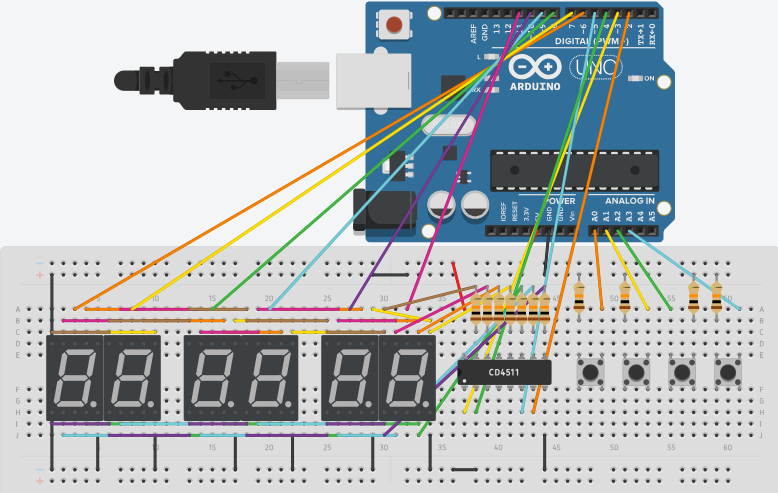
\includegraphics[width=0.6\textwidth]{figs/Clock_Tinkercad.png}
\caption{Clock Tinkercad Simulation}
\end{frame}

\section{Conclusion}
\begin{frame}{Summary}
\begin{itemize}
    \item Successfully implemented digital clock with editing features
    \item Efficient multiplexing and minimal I/O usage
    \item Complete increment/decrement logic implemented via Boolean expressions
    \item Full digit-by-digit editing with constraints for hours, minutes, seconds
\end{itemize}
\end{frame}

\begin{frame}{Acknowledgment}
\centering
The complete source code and documentation can be found at:\\
\url{https://github.com/Dhawal24112006/projects.git}

\vspace{1cm}
Thank You!
\end{frame}

\end{document}

